\chapter{Cơ sở lý thuyết}
\label{chap:background}

\section{Ca kiểm thử, miền đầu vào và oracle}
\label{sec:testing-concepts}

Với một hàm, ca kiểm thử ghi bộ đối số và đầu ra mong đợi~\cite[tr.~7--8]{pham2014kiemthu}. Cặp ngày 31, tháng 4 cho thấy vì sao kiểm riêng từng đối số chưa đủ. Hai giá trị đều là số nguyên, nhưng kết hợp lại thì nằm ngoài miền ngày hợp lệ. \textit{Test oracle} đối chiếu kết quả thực tế với yêu cầu của bài~\cite{istqb2024}.

HumanEval đưa ra đặc tả và bộ test cơ sở cho mỗi bài Python. HumanEval+ của EvalPlus thêm test để phân biệt những cài đặt cùng vượt bộ ban đầu. Trong khóa luận, cài đặt tham chiếu HumanEval+ cho biết kết quả mong đợi của các bộ đối số mới~\cite{chen2021evaluating,liu2023evalplus}.

\section{Kiểm thử chức năng}
\label{sec:functional-techniques}

Kiểm thử chức năng lấy hành vi trong đặc tả làm căn cứ chọn ca. Theo cách tiếp cận hộp đen, người kiểm thử xác định giá trị cần đưa vào và kết quả cần quan sát từ các quy tắc của bài. Do đó, một bộ ca có thể dùng cho nhiều cài đặt cùng đặc tả~\cite[tr.~12--14]{pham2014kiemthu}.

\subsection{Phân hoạch tương đương}

Phân hoạch tương đương (EP) chia miền thành các lớp rời nhau. Các giá trị trong cùng một lớp tuân theo cùng quy tắc xử lý, nên có thể chọn một giá trị đại diện để thử. Cần tách lớp khi tìm thấy điều kiện làm thay đổi quy tắc cần kiểm~\cite[tr.~131--133]{pham2014kiemthu}.

Hai chuỗi \texttt{"a b"} và \texttt{"a,b"} dài bằng nhau. Chuỗi đầu đại diện cho lớp tách theo khoảng trắng, còn chuỗi thứ hai đại diện cho lớp có dấu phẩy và thiếu khoảng trắng. \texttt{"abc"} thuộc lớp thứ ba vì thiếu cả hai dấu phân cách.

\subsection{Phân tích giá trị biên}

BVA thông thường lấy một bộ đối số danh định làm mốc, tức các giá trị điển hình trong miền. Giữ những đối số khác như cũ, rồi lần lượt đưa đại lượng đang xét về hai cận và hai giá trị kề phía trong. Một lỗi so sánh lệch một đơn vị có thể chỉ xuất hiện ở các mốc này~\cite[tr.~122--126]{pham2014kiemthu}.

Với tháng \(m\) trong khoảng từ 1 đến 12, giữ ngày 15 và cùng một năm. Lấy tháng 6 làm mốc, sau đó thử 1, 2, 11 và 12. Nếu trong mã dùng \(m < 12\) thay cho \(m \le 12\), ca tháng 12 sẽ làm lộ lỗi. Khi các đối số phụ thuộc nhau, phải kiểm lại cả bộ sau mỗi thay đổi. Giữ ngày 31 rồi đổi tháng sang 4 sẽ ra ngoài miền. Biến thể kiểm thử giá trị biên mạnh (\textit{robust BVA}) còn dùng 0 và 13 để kiểm cách xử lý tháng ngoài miền theo đặc tả~\cite[tr.~123--126]{pham2014kiemthu}.

\subsection{Kiểm thử bằng bảng quyết định}

Một cột trong bảng quyết định (DT) ghi một tổ hợp điều kiện và hành động phải thực hiện khi tổ hợp đó xảy ra. Muốn biến cột thành ca kiểm thử, cần tìm một đầu vào thỏa các điều kiện rồi quan sát xem hàm có thực hiện đúng hành động ghi trong cột hay không~\cite[tr.~141--144]{pham2014kiemthu}.

Ở Bảng~\ref{tab:word-split-rules}, cả hai tổ hợp có khoảng trắng đều tách theo khoảng trắng, bất kể có dấu phẩy hay không. Hai tổ hợp vì thế được ghi chung trong cột \(R_1\). Dấu gạch biểu thị điều kiện có thể nhận cả hai giá trị~\cite{istqb2024}. Với \(R_3\), hàm đếm chữ cái thường có chỉ số lẻ, bắt đầu đánh số từ \texttt{a} ở vị trí 0.

\begin{table}[!htbp]
\centering
\caption{Bảng quyết định cho bài toán tách từ của HumanEval}
\label{tab:word-split-rules}
\small
\begin{tabular}{@{}lccc@{}}
\toprule
 & \(R_1\) & \(R_2\) & \(R_3\) \\
\midrule
Có khoảng trắng & Có & Không & Không \\
Có dấu phẩy & \textemdash & Có & Không \\
Hành động & \makecell{Tách theo\\khoảng trắng} & \makecell{Tách theo\\dấu phẩy} & \makecell{Đếm chữ thường\\có chỉ số lẻ} \\
Đầu vào đại diện & \texttt{"a b"} & \texttt{"a,b"} & \texttt{"abc"} \\
\bottomrule
\end{tabular}
\end{table}

\section{Kiểm thử luồng điều khiển}
\label{sec:control-flow-theory}

\subsection{Đồ thị luồng điều khiển (CFG)}

Trong đồ thị luồng điều khiển (\textit{control-flow graph}, CFG), mỗi đỉnh là một câu lệnh hoặc một nhóm lệnh chạy liền nhau. Cạnh hướng tới vị trí chương trình có thể chạy tiếp. Một điểm quyết định có một cạnh cho mỗi kết quả của điều kiện. Đường từ đỉnh vào đến đỉnh ra mô tả một thứ tự thực thi có thể có. Để đi đúng đường đó, đầu vào phải thỏa các điều kiện ở những điểm rẽ dọc đường~\cite[tr.~156--158]{pham2014kiemthu}.

Hình~\ref{fig:cfg-dfg} dùng một hàm nhận \(x\) và trả \texttt{kq}. Nửa trái cho thấy biến được khởi tạo bằng 0 và chỉ đổi khi \(x > 0\). Truyền \(x = 1\) thì phần thân chạy qua \(1\to2\to3\to4\). Với \(x = 0\), chương trình đi thẳng theo cạnh \(2\to4\), bỏ qua phép gán thứ hai.

\begin{figure}[!htbp]
\centering
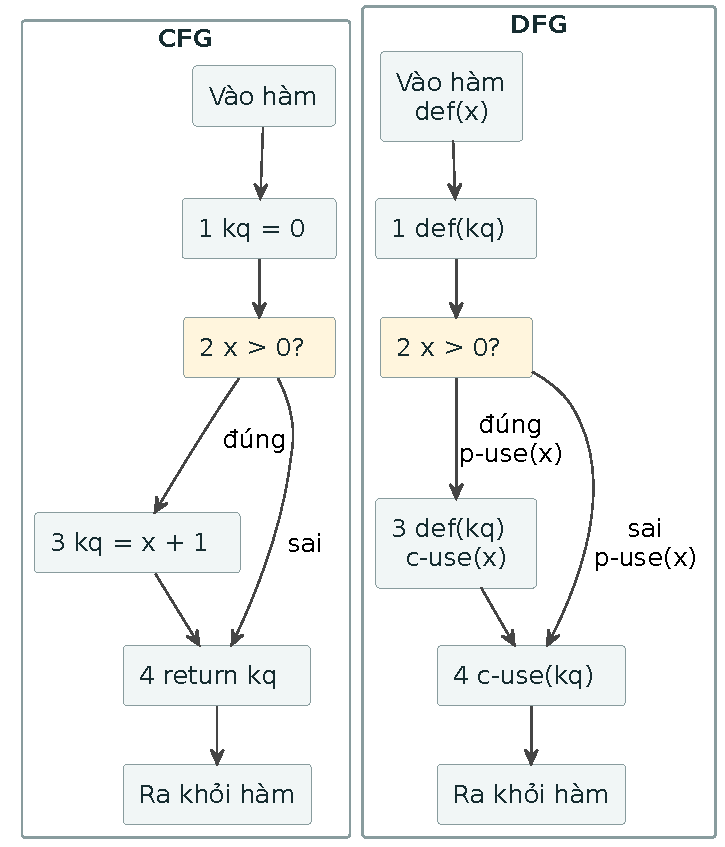
\includegraphics[width=.89\linewidth,height=.45\textheight,keepaspectratio]{diagrams/cfg-dfg.pdf}
\caption{CFG và DFG của một hàm có một nhánh. Các số 1 đến 4 chỉ cùng vị trí trong mã.}
\label{fig:cfg-dfg}
\end{figure}

\subsection{Độ phủ câu lệnh và độ phủ nhánh}

Ca \(x = 1\) chạy cả bốn dòng, nên ví dụ đã đủ C1. Để đạt C2, cần quan sát cả hai kết quả của quyết định ở dòng 2. Thêm ca \(x = 0\) sẽ đi qua cạnh sai. Nếu điều kiện được ghép từ nhiều điều kiện con, có đủ hai lối ra vẫn chưa cho biết từng điều kiện con đã được đánh giá với những giá trị nào~\cite[tr.~158--160]{pham2014kiemthu}.

ConceptTester dùng dòng thực thi để xấp xỉ C1 và dùng cạnh chuyển dòng để đo C2~\cite{coverageBranchDocs}. Từ mã nguồn, công cụ tìm các cạnh có thể đi. Nếu trace của test cơ sở thiếu một cạnh trong số đó, ControlFlow có thể chọn cạnh ấy làm đích sinh đầu vào ở Chương~\ref{chap:method}.

\section{Kiểm thử luồng dữ liệu}
\label{sec:data-flow-theory}

\subsection{Đồ thị luồng dữ liệu (DFG)}

Đồ thị luồng dữ liệu (\textit{data-flow graph}, DFG) gắn thông tin về biến lên đường thực thi. Theo cách biểu diễn trong giáo trình, đỉnh ghi nơi biến nhận giá trị (\textit{def}) hoặc được đọc để tính toán hay trả kết quả (\textit{c-use}). Nếu điều kiện rẽ nhánh đọc một biến, \textit{p-use} của biến được ghi trên cạnh tương ứng. Tham số nhận giá trị ở đỉnh vào hàm~\cite[tr.~189--195]{pham2014kiemthu}.

Ở nửa phải Hình~\ref{fig:cfg-dfg}, cả hai cạnh ra từ dòng 2 mang nhãn \texttt{p-use(x)} vì hàm phải biết \(x\) mới chọn được lối đi. Dòng 3 đọc \(x\) khi tính \(x+1\), rồi ghi kết quả vào \texttt{kq}. Dòng 4 đọc \texttt{kq} để trả về. Các nhãn này cho phép lần ngược giá trị được đọc về phép gán đã tạo ra nó.

\subsection{Cặp định nghĩa và sử dụng (def--use)}

Một lần gán và một lần đọc tạo thành cặp def--use nếu giá trị của phép gán tới được chỗ đọc. Điều này đòi hỏi biến chưa bị gán lại ở đoạn giữa. Giáo trình gọi đường đi như vậy là \textit{def-clear}~\cite[tr.~193--195]{pham2014kiemthu}.

Với \(x = 1\), dòng 3 thay giá trị của \texttt{kq}, nên dòng 4 nhận giá trị từ dòng 3. Với \(x = 0\), đường chạy bỏ qua dòng 3 và giữ giá trị ở dòng 1. Ca đầu tiên đủ phủ câu lệnh. Ca thứ hai cần để thấy cặp \(1\to4\) của \texttt{kq}.

Theo \textit{all-defs}, mỗi lần gán có thể tới một chỗ sử dụng cần ít nhất một ca đưa giá trị đến một chỗ như vậy. \textit{all-uses} yêu cầu phủ từng cặp gán và sử dụng khả thi~\cite[tr.~197--201]{pham2014kiemthu}. Trong thực nghiệm, ControlFlow dùng cặp def--use tĩnh để gợi ý phép gán nào có thể đưa giá trị tới dòng cần thử. Trace kiểm tra xem input đi qua dòng hay cạnh nào. Oracle đối chiếu đầu ra.

\section{Công cụ sử dụng}
\label{sec:related-technologies}

Trong các lần chạy được báo cáo, \textit{coverage.py} ghi dòng và cạnh để ControlFlow tìm vị trí còn thiếu, còn \textit{python-graphs} cung cấp quan hệ truy cập biến từ đồ thị của mã Python. Nếu mô hình mô tả miền lấy mẫu, Hypothesis lấy thêm giá trị từ miền đó~\cite{coverageBranchDocs,pythonGraphs,hypothesisIntroDocs}.

Trước lúc chạy PUT, Pydantic kiểm cấu trúc dữ liệu trả về và Bubblewrap cô lập tiến trình Python. Prefect ghi cấu hình và trạng thái của lần chạy để có thể tra lại kết quả~\cite{pydanticModelsDocs,bubblewrapDocs,prefectFlowsDocs}.

\section{Nghiên cứu liên quan}
\label{sec:related-work}

SDART của Nguyễn Đức Anh và cộng sự tìm thêm dữ liệu kiểm thử C++ bằng phân tích tĩnh khi chiến lược chọn đường khó phủ thêm nhánh~\cite{nguyen2019sdart}. Hai nghiên cứu sau đưa mô hình ngôn ngữ vào kiểm thử concolic theo các cách khác nhau. ConAgent dùng tác tử LLM để khởi tạo đối tượng Qt và sinh dữ liệu cho đường chứa lệnh chưa phủ~\cite{trong2026conagent}. ConAI chạy concolic rồi dùng mô hình nhỏ đã tinh chỉnh để sinh thêm input cho các đường được chọn~\cite{tran2026conai}.

SymPrompt đưa đường thực thi vào prompt. CoverUp chọn dòng hoặc nhánh chưa phủ rồi đưa phản hồi từ lượt chạy trước vào lần sửa test~\cite{ryan2024symprompt,pizzorno2025coverup}. DeepMOSA dùng thuật toán di truyền trên Python và gọi mô hình ngôn ngữ cho các nhánh còn thiếu khi độ phủ ngừng tăng~\cite{dao2026deepmosa}. ConceptTester cũng lấy độ phủ để tìm vị trí nên thử. Khi phân tích kết quả, khóa luận đếm số PUT cho đầu ra khác tham chiếu.

Mathews và Nagappan ghi nhận trường hợp oracle chấp nhận hành vi sai của chương trình~\cite{mathews2024design}. Để bước chấm độc lập với giả định của mô hình sinh test, ConceptTester chốt input trước khi chạy tham chiếu. Số PUT bị phát hiện chỉ tính những sai khác đã được xác nhận.
